\section{Reformas dos Setores Elétricos}

\subsection{Introdução}
    Nesta aula abordaremos as reformas dos setores elétricos, onde inicialmente todos operavam e planejavam o sistema, onde o governo regia o setor elétrico em todos os âmbitos de maneira vertical , sendo representado por uma estatal que no caso do Brasil será a Eletrobrás.
    O problema da verticalização é que como o setor elétrico tem um grau elevado de importância para a economia e pelo fato de ser fruto de grande ineficiência quando administrado de maneira vertical, podem ser causados danos imensuráveis para a sociedade uma vez que temos grandes ineficiências e pouca capacidade de inovação. Pelo fato da capacidade de evolução da sociedade está atrelada a capacidade de obter energia e possuir um custo mais barato de energia então, irá fomentar industrias mais competitivas que permitem ter investimentos e assim fazer com que a economia cresça. Se o custo de energia permanecer alto nenhuma indústria irá se instalar e nem ocorrerá instalações de polos industriais em determinadas regiões, criando assim uma economia estagnada gerando impactos sociais.
    
\subsection{Reforma dos setores elétricos}
  A eletricidade é um serviço estrutural, ou seja estrutura todo o resto da economia.Hoje em dia a economia e a resto da sociedade está ligada à eletricidade, por exemplo se não houvesse eletricidade não teríamos iluminação,industria, celulares, etc. setor elétrico demanda uma grande quantidade de investimentos ou seja é necessários novos investimentos principalmente em países onde ocorre o crescimento da demanda.Se crescêssemos 4\% ao ano teríamos,em 15 anos, que dobrar o sistema inteiro, onde isso é quase impossível de acontecer pelo curto intervalo de tempo e o alto investimento da construção. Se pensássemos de maneira quantitativa, uma hidroelétrica demora5 5 anos para ser construído,ou seja ocorreria três grandes
ciclos de construções de hidroelétrica. Estes investimentos devem ser realizados de maneira eficiente e de maneira adaptativa com a realidade econômica do país.
\begin{figure}[H]
\begin{centering}
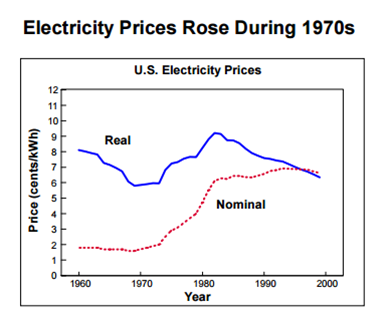
\includegraphics[scale=0.6]{aula9_1}\protect\caption{\label{fig:aula9-1} Preço da eletricidade EUA 1970}
\end{centering}
\end{figure}

  A figura \ref{fig:aula9-1} apresenta o aumento de preço da preço da eletricidade à partir de 1970. Então nos anos 70 a estrutura verticalizada e administrada pelo setor público passa ser desafiada. Como principal motivo o aumento dos preços dos combustíveis na crise do petróleo e todo o setor estava despreparado para enfrentar uma crise, desafiando assim a estrutura do setor.Além da crise do petróleo,o limite da economia de escala estava esgotada e a incapacidade gerencial das empresas públicas de reagir começaram a ter problemas não tendo poder financeiro de reação. Esses motivos levaram a uma crise sem rescendentes nos EUA na época de 70 a 80, gerando a falência das empresas que foram construídas para supri a cadeia necessária para sustentar o setor elétrico
  Para contornar a crise ocorrem investimentos em pequenos geradores, onde uma grande quantidade de geradores foram instaladas. Assim, a reação que o setor privador poderia contribuir para contornar a crise gerou uma nova perspectiva e visão que o mercado poderia atrair investimentos eficientes e mostrando que essas centenas de geradores instalados cobriram o deficit de carga daquele momento.
  A primeira mudança foi a privatização,onde  houve um consenso que setor público era menos eficiente em reagir adaptativamente a mudanças e inovações de maneira do que o setor privado. Para trazer capital externo para manter o setor elétrico em tempo hábil com eficiência e com inovação teria que ser capital externo se não poderia gerar um deficit público, E poder ter agentes privados dentro do setor elétrico foi criado uma ambiente competitivo.Assim, a primeira medida para a reestruturação foi a desverticalização.
  De maneira geral, separando a geração, a distribuição e a transmissão.Sendo que a competição será no segmento da geração, onde a geração começa fica aberta para novos investimentos privados.
   A ideia de energia como uma commodity, inicialmente era tratar a eletricidade da mesma forma como outras indústrias em que as forças do mercados guiam o processo. Onde a demanda dita a oferta de preço do mercado e a quantidade. Assim, a rede de transmissão trsnporta a commodity, conforme apresentado da figura(\ref{fig:aula9-2}).
\begin{figure}[H]
\begin{centering}
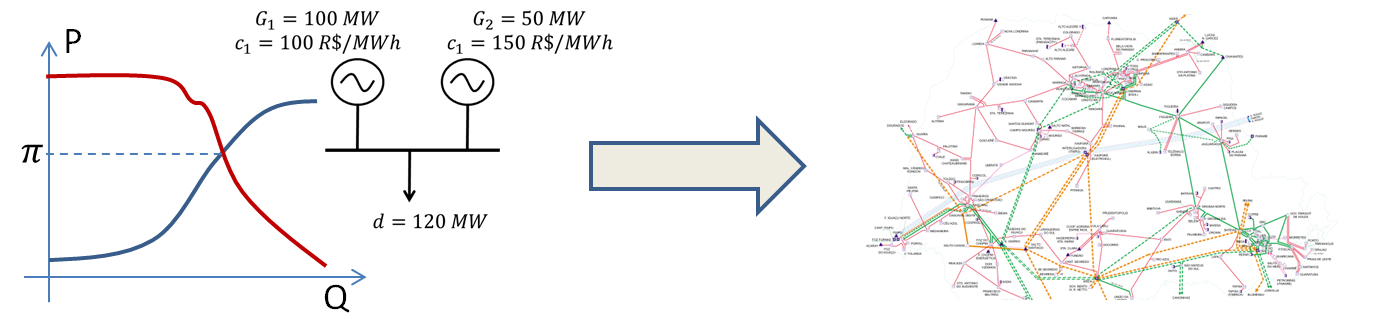
\includegraphics[scale=0.6]{aula9_2}\protect\caption{\label{fig:aula9-2} Energia como uma commodity }
\end{centering}
\end{figure}
  A energia é um serviço, até as tecnologias evoluírem esse conceito de energia se manterá. Existem uma série de particularidades que devem ser levadas em consideração que limitam esse serviço e pode ser dividido entre os aspectos tecnológicos e sistêmicos. No aspectos tecnológico podemos citar, as rampas dos gerados onde não é possível aumentar a potencia de uma hora para outra, existem também as restrições tecnológicas de máximo e mínimo tempo desligados e ligados do gerados e restrições complexas interação da rede (segunda lei de  Kirchhoff) e do aspecto da incapacidade de estocar e transportar a energia estocada. Nos aspectos sistêmicos é verificado o compartilhamento de recursos hídricos quanto existem usinas em cascatas num rio a quantidade turbinada pela primeira usina modificada o insumo da outra usina e a confiabilidade e segurança de suprimento. Pode-se concluir que o desenho do mercado a ser instalado depende das características do sistema.
  No sentido de criar uma desregulamentação e proporcionar toda essa modificação, ocorreu a criação de novas instituições. A primeira instituição a ser criada foi o operador do sistema como empresa independente do governo pelo fato de ter incentivos econômicos alinhados com a eficiência do sistema de suprimento. A segunda entidade é operador do mercado pelo fato de existir uma grande conexão entre o mercado e as transações feitas entre gerados e consumidores. Por último temos a criação do regulador que ter por objetivo monitorar e regular o operador de mercado e o operador do sistema, na figura \ref{fig:aula9-3} está ilustrada esse esquema de mercado.

\begin{figure}[H]
\begin{centering}
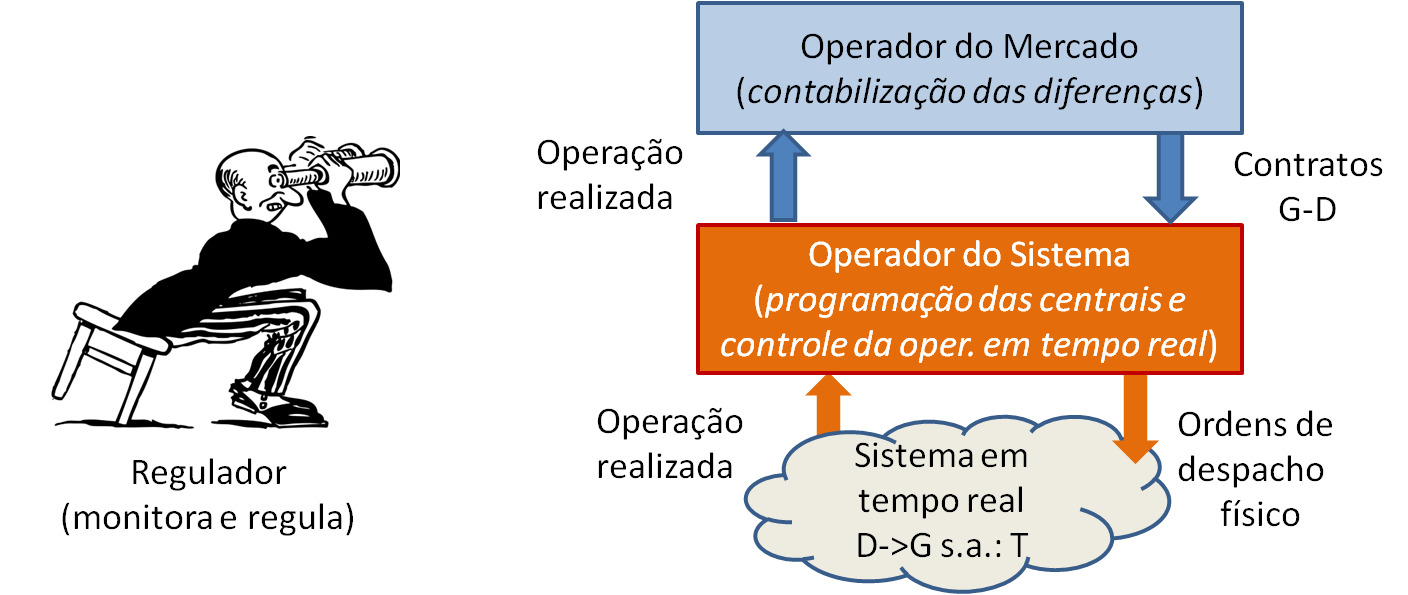
\includegraphics[scale=0.4]{aula9_3}\protect\caption{\label{fig:aula9-3} Esquema do mercado }
\end{centering}
\end{figure}
\subsection{Reforma no Brasil}

 A reforma teve inicio no Brasil em 1996, aproximadamente 16 anos depois dos EUA, e teve como finalidade de encorajar a entrada de novos participantes no mercado para isso encorajando a competição no segmento da geração e a distribuição e transmissão continuaram regulados. Então, foram foram criados os principais órgãos, o operado nacional do sistema (ONS), o operador do mercado que no brasil foi chamado de mercado atacadista de energia (MAE) e regulador que foi intitulada de Agencia Nacional de Energia Elétrica (ANNEL) que além de observar o movimento da ONS e MAE, cria as regulamentações, regula e inspeciona o sistema. E neste instante foi criada a ideia de contratos bilaterais estabelecidos entre geradores e distribuidores para isso ocorre uma série de desverticalização dentro das empresas.
 \begin{figure}[H]
\begin{centering}

\includegraphics[scale=1]{aula9_5}\protect\caption{\label{fig:aula9-5} Crise energética 2002}
\end{centering}
\end{figure}

 Em 2002, o Brasil entrou numa enorme crise energética conhecida como "apagão", que afetou o fornecimento e distribuição de energia e apontou pela falta de planejamento e investimento do governo em relação ao setor elétrico. A principal causa foi a falta de chuva que teve como consequência diminuição do nível de água dos reservatórios das hidroelétricas conforme mostrado no gráfico da figura \ref{fig:aula9-4}  levando a um racionamento de energia.
 
\begin{figure}[H]
\begin{centering}
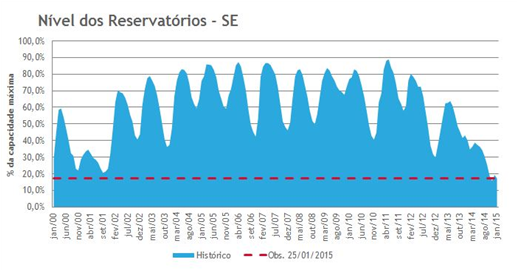
\includegraphics[scale=1]{aula9_4}\protect\caption{\label{fig:aula9-4} Nível dos reservatórios na época da crise energética de 2002 }
\end{centering}
\end{figure}

 Pela falta de planejamento e investimento do governo algumas questões foram levantadas, como garantir a sustentabilidade do sistema de logo prazo e como desenhar um mercado que seja capaz de atrair investimento em tempo para suprir uma demanda sempre crescente. A resposta dessas questões serão respondidas na aula 11, onde será apresentada a ampla reforma realizada em 2004.
  A operação pode ser coordenada de diversas maneiras, por exemplo um simples preço determinado pelo operador de remuneração para os geradores produzindo ou os geradores se acoplam e desacoplam de acordo com suas percepções do preço futuro. Ou seja,a frequência do sistema dita o preço. A frequência em queda menos a potencia gerada deve ser menor que a demanda, assim o operador aumento o preço e atrai mais geração e eventualmente atraindo
geradores off-line a se acoplarem à rede. A elevação da frequência menos a potencia de geração deve ser maior que a demanda, assim operador diminui o preço incentivando a redução da injeção de potencia eventualmente desacoplando geradores da rede, apresentado na figura \ref{fig:aula9-6}.

\begin{figure}[H]
\begin{centering}
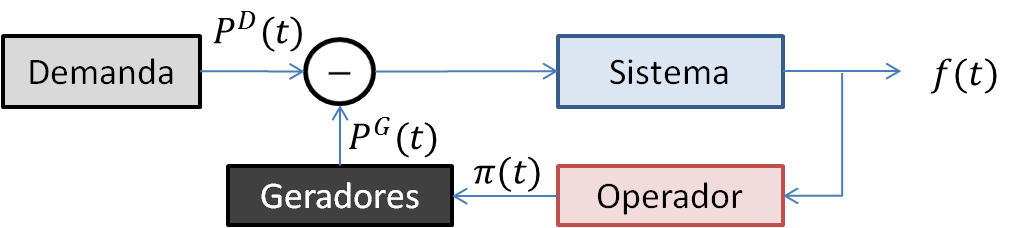
\includegraphics[scale=0.6]{aula9_6}\protect\caption{\label{fig:aula9-6} Esquema do sistema }
\end{centering}
\end{figure}

 A possibilidade de muitas externalidades tornam esse processo ineficiente ocorrendo: complexas interações entre a rede e os geradores e demanda, contingencias, custos e restrições não triviais de serem recuperados (start up, shut down, munimum up e down time).
O planejamento do uso ótima dos recursos disponíveis traz eficiência
Para uma planejamento do uso ótimo dos recursos disponíveis tem vinculado o unit commitment,a analise de contingencias e despacho econômico com segurança.Assim, esse processo de planejamento vai do longo ao curtíssimo prazo e passa a controlar o uso dos recursos e determinar o preço de curto prazo (spot) gerando intensivo do uso de ferramentas de otimização e estatística.

\subsection{Planejamento do setor}
  Um conceito importante para o planejamento do setor é o preço de spot ($\pi$), que é o preço do recurso mais caro necessário para fazer a geração atender à demanda. Este preço deve refletir o ``máximo necessário'' da operação em tempo real. Para isso pode-se determinar o preço marginal da operação através de um processo ex-ante ou de um processo ex-post. O preço de spot obtido ex-ante pelo modelo de despacho de mais curto prazo possui eventuais diferenças entre operação real e planejada que tornam-se encargos outro ponto importante é que preços ex-ante tendem a ser menos voláteis e mais ``previsíveis'' que no esquema ex-post. O obtido ex-post, pela operação real gera preços excessivamente voláteis que podem penalizar muito consumidores específicos e reduzir a atratividade do mercado. No Brasil utiliza-se o ex-ante em etapas semanais e diversas diferenças da operação de tempo real são contabilizadas como encargos de serviço e sistema (ESS).
  O despacho conforme mencionado anteriormente é programação dos recursos para próxima hora, dia ou mês. Existem duas maneira de realizar o despacho por custo onde o operador calcula o custo de oportunidade da água através de um modelo computacional que simula a operação do sistema em diversas condições conforme a figura \ref{fig:aula9-7} que calcula-se a função de custo futuro de maneira computacional.Ou outra forma de despacho é por oferta que o operador recebe ofertas de preço e a quantidade dos geradores baseado
na percepção privada de cada agente sobre o sistema,seus recursos,economia,etc. Em ambos os casos o despacho é realizado pelo operador objetivando a atender a demanda ao menor custo 
respeitando as restrições de rede,tecnologia e confiabilidade.
\begin{figure}[H]
\begin{centering}
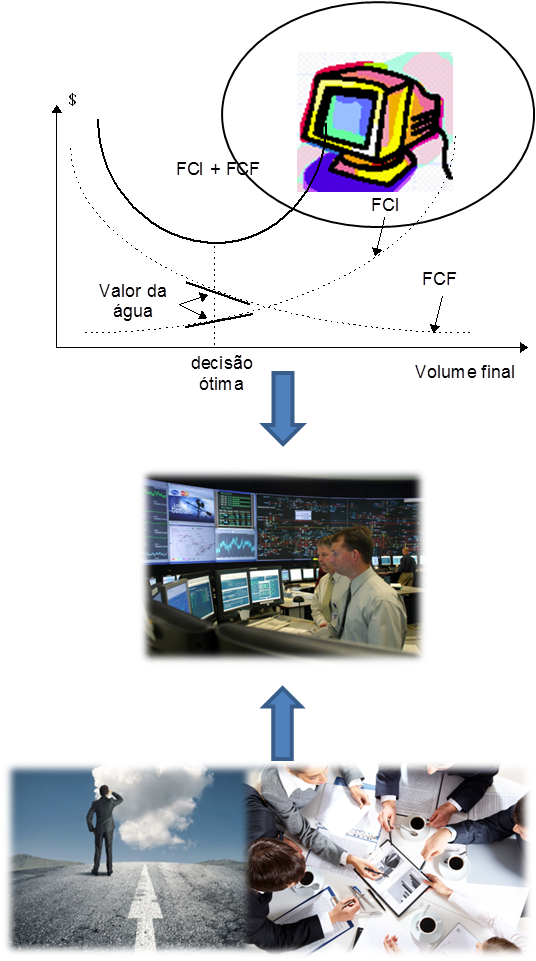
\includegraphics[scale=0.5]{aula9_7}\protect\caption{\label{fig:aula9-7} Despacho por custos }
\end{centering}
\end{figure}
 O preço Spot no Brasil, é calculado por um sistema onde temos o NEWAVE que faz basicamente o cálculo da função de custo futuro e a função de custo imediato realiza uma simulação e aplica a programação dinâmica dual estocástica, esta realização é realizada mensalmente. Através dos dados tratos pelo NEWAVE é realizado o input no modelo DECOMP que é realizado em escala semanal que tem como objetivo tratas as restrições elétricas. Assim os dados são analisados e ocorre a publicação dos preço onde,os valores de PLD são calculados toda sexta feira e publicados no site da CCEE, www.ccee.org.br. Este esquema esta apresentado na figura \ref{fig:aula9-8}.

\begin{figure}[H]
\begin{centering}
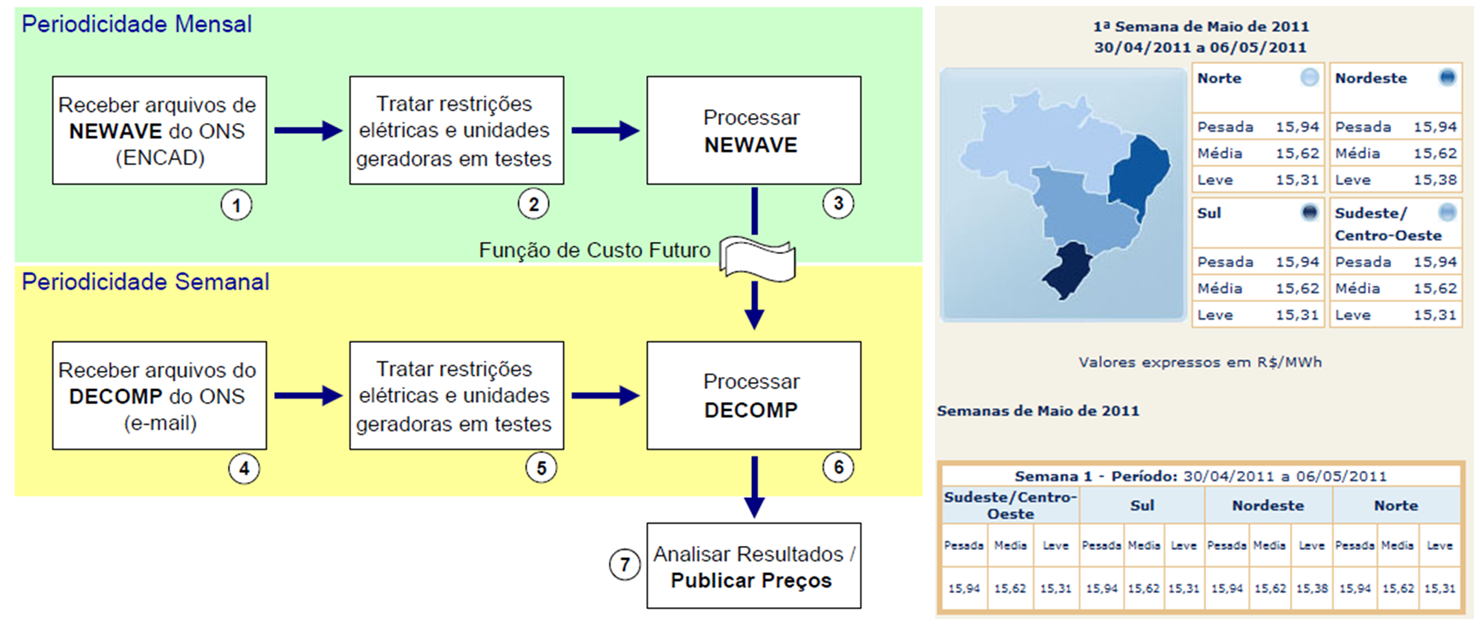
\includegraphics[scale=0.5]{aula9_8}\protect\caption{\label{fig:aula9-8} Preço Spot no Brasil }
\end{centering}
\end{figure}

Considerando um exemplo simples, onde temos 3 geradores com limites de geração iguais a 10MWh,5MWh e 20MWh respectivamente. Então temos que,
\begin{align}
    & z={\text{Min}} \hspace{1cm} 8g_{1}+12g_{1}+15g_{3} \\
    & \text{s.a}  \hspace{2.2cm}   g_{1}+g_{1}+g_{3} \\
    &             \hspace{2.65cm} g_{1}\leq 10 \\
    &             \hspace{2.65cm} g_{2}\leq 5 \\
    &             \hspace{2.65cm} g_{3}\leq 20 \\
\end{align}
\\$\pi=\frac{\partial z}{\partial D}=12.$\\
O preço de spot desse exemplo é 12, ou seja a variável associada a restrição dual do problema.
Um ponto interessante é que solução ótima não impõe uma perda marginal de produção. Conforme mostrado a seguir:

$R_{i}=(\pi-c_{i})\cdot g_{i}\geq0$, pois $g_{i}=0$ se $\pi<c_{i}$

$$R_{1}=(12-8)\cdot10=40$$

$$R_{2}=(12-12)\cdot4=0$$

$$R_{1}=(12-15)\cdot0=0.$$


Então a receita no mercado atacadista os geradores são creditados pela sua geração ao valor do preço spot de sua região ou barra dado por:

$$R_{it}^{MAE}=g_{it}\cdot\pi_{it}$$
 Assim, todos os geradores que produzem possuem lucro marginal e dependendo da forma que o mercado determina o preço (mais ou menos realismos), geradores podem ou não recuperar todos os custos. Quanto mais simplificado o mercado mais o gerador tem a chance de
não recuperar custos de acionamento. POOL vs Exchange Markets
Voltando ao exemplo anterior, se existir um custo de acionamento, o gerador
$1$e $2$ poderiam perder dinheiro então, suponha um custo fixo de acionamento de $50\$$ igual para todos os geradores e supondo dois período, temos que:
Para $t=1:$ $R_{11}=(12-8)\cdot10-50=-10$ $R_{2}=(12-12)\cdot4-50=-50$
Para $t=2:$ $R_{12}=(12-8)\cdot10=+40$ $R_{2}=(12-12)\cdot4=0$
Total: $R_{11}+R_{12}=+30$ $R_{21}+R_{22}=-50.$
Suponha duas barras e os mesmos geradores, só que o gerador 1 está em uma barra e os geradores 2 e 3 ficaram na outra barra, a demanda também foi dividida por barra. O exemplo possui os mesmos valores do exemplo anterior,apenas foi adicionada uma barra de transmissão (conforme apresentado na figura \ref{fig:aula9-9}. Então a modelagem será dada por:

\begin{align}
    & z={\text{Min}} \hspace{1cm} 8g_{1}+12g_{1}+15g_{3} \\
    & \text{s.a}  \hspace{2.2cm}   g_{1}-f=3 \\
    &             \hspace{2.65cm} g_{2}-g_{3}=3 \\
    &             \hspace{2.65cm} |f|\leq + \infty \\
    &             \hspace{2.65cm} g_{1}\leq 10 \\
    &             \hspace{2.65cm} g_{2}\leq 5 \\
    &             \hspace{2.65cm} g_{3}\leq 20. \\
    \end{align}
\begin{figure}[H]
\begin{centering}
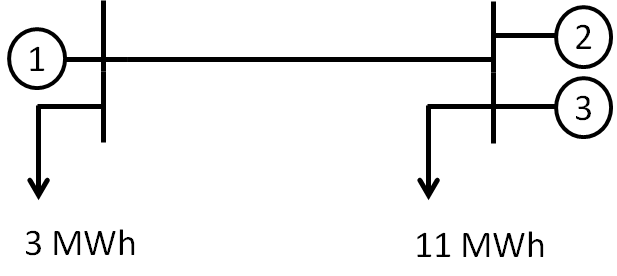
\includegraphics[scale=0.5]{aula9_9}\protect\caption{\label{fig:aula9-9} Exemplo linha de transmissão}
\end{centering}
\end{figure}
O custo marginal em cada barra será, $\pi_{A}=\pi_{B}=12\$/MWh$ e o despacho ótimo é dado pela figura  \ref{fig:aula9-10}.
\begin{figure}[H]
\begin{centering}
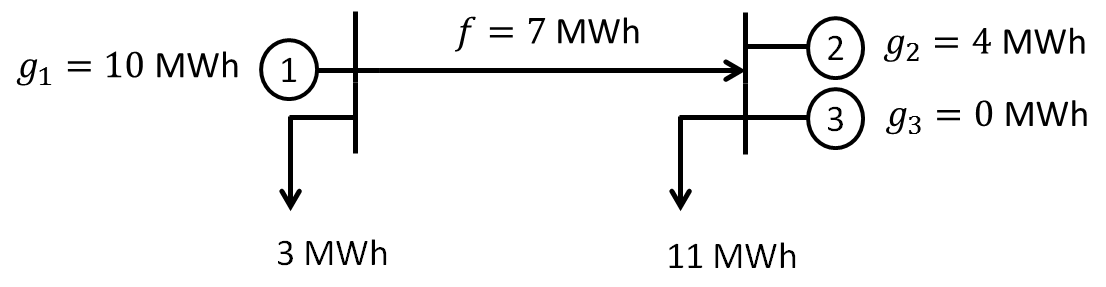
\includegraphics[scale=0.5]{aula9_10}\protect\caption{\label{fig:aula9-10} Despacho ótimo exemplo da linha de transmissão }
\end{centering}
\end{figure}
A tabela abaixo representa a contabilização no mercado de curto prazo do exemplo da transmissão.

\begin{tabular}{|c|c|c|c|c|}
\hline 
 & Geração g MWh & Consumo D MWh & Spot $\pi$$\$/MWh$ & Receita/Despesa $g\times\pi$ou $-D\times\pi$ $\$$\tabularnewline
\hline 
\hline 
$G_{1}$ & 10 &  & 12 & $10\times12=120$\tabularnewline
\hline 
$G_{2}$ & 4 &  & 12 & $4\times12=48$\tabularnewline
\hline 
$G_{3}$ & 0 &  & 12 & 0\tabularnewline
\hline 
$D_{1}$ &  & 3 & 12 & $-3\times12=-36$\tabularnewline
\hline 
$D_{2}$ &  & 11 & 12 & $-11\times12=-132$\tabularnewline
\hline 
Fechamento & 14 & 14 & 12 & $(14-14)\times12=0$\tabularnewline
\hline 

\end{tabular}



Modificando o exemplo, colocando um limite de fluxo na linha de transmissão apresentado na figura \ref{fig:aula9-10}. E a modelagem dada por:
\begin{align}
    & z={\text{Min}} \hspace{1cm} 8g_{1}+12g_{1}+15g_{3} \\
    & \text{s.a}  \hspace{2.2cm}   g_{1}-f=3 \\
    &             \hspace{2.65cm} g_{2}-g_{3}=3 \\
    &             \hspace{2.65cm} |f|\leq 5\\
    &             \hspace{2.65cm} g_{1}\leq 10 \\
    &             \hspace{2.65cm} g_{2}\leq 5 \\
    &             \hspace{2.65cm} g_{3}\leq 20. \\
    \end{align}
\begin{figure}[H]
\begin{centering}
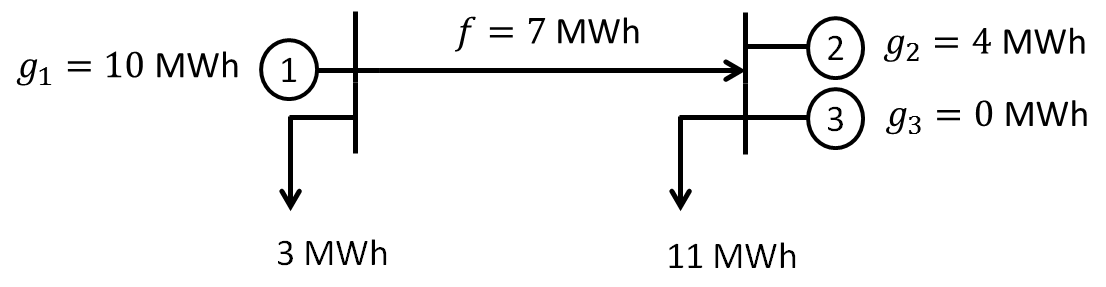
\includegraphics[scale=0.5]{aula9_10}\protect\caption{\label{fig:aula9-10} Exemplo linha de transmissão com limite de fluxo}
\end{centering}
\end{figure}

Agora o preço de spot foi modificado em cada barra, na primeira barra $\pi_{A}=8\$/MWh$
 e na segunda barra $\pi_{B}=15\$/MWh$ e o despacho ótimo dado pela figura \ref{fig:aula9-11}
 
 \begin{figure}[H]
\begin{centering}
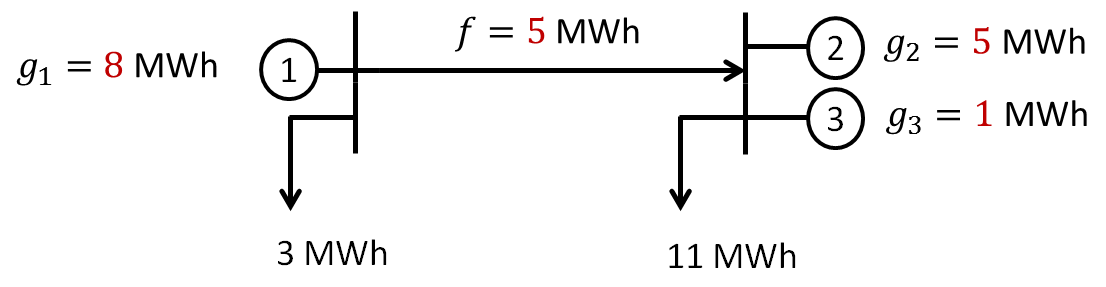
\includegraphics[scale=0.5]{aula9_11}\protect\caption{\label{fig:aula9-11} Exemplo despacho ótimo linha de transmissão com limite de fluxo}
\end{centering}
\end{figure}
A tabela abaixo representa a contabilização no mercado de curto prazo do exemplo da transmissão com limite na linha.
\begin{tabular}{|c|c|c|c|c|}

\hline 
 & Geração g MWh & Consumo D MWh & Spot $\pi$$\$/MWh$ & Receita/Despesa $g\times\pi$ou $-D\times\pi$ $\$$\tabularnewline
\hline 
\hline 
$G_{1}$ & 8 &  & 8 & $8\times8=64$\tabularnewline
\hline 
$G_{2}$ & 5 &  & 15 & $5\times15=75$\tabularnewline
\hline 
$G_{3}$ & 1 &  & 15 & $1\times15=75$\tabularnewline
\hline 
$D_{1}$ &  & 3 & 8 & $-3\times8=-24$\tabularnewline
\hline 
$D_{2}$ &  & 11 & 15 & $-11\times15=-165$\tabularnewline
\hline 
Fechamento & 14 & 14 &  & $soma=-35$\tabularnewline
\hline 

\end{tabular}

 O sinal para a expansão onde construímos uma sistema,o crescimento da demanda passa a exigir a utilização de recursos mais caros,a expectativa de preços futuros se eleva e novos geradores se instalam buscando lucrar com o atendimento à demanda.
 A figura /ref{fig:aula9-15} abaixo representa o preço de spot e mostra a relação da curva de geração com a curva de demanda futura e a variação do preço de spot.

 \begin{figure}[H]
\begin{centering}
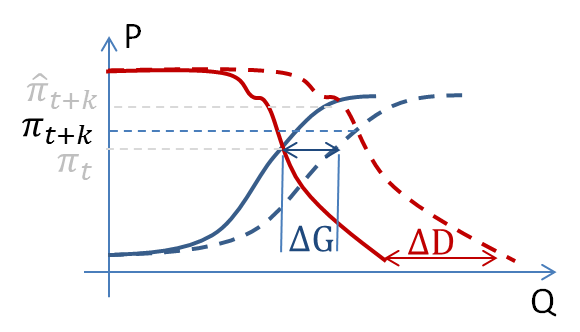
\includegraphics[scale=0.5]{aula9_15}\protect\caption{\label{fig:aula9-15} curva demanda Xpreço}
\end{centering}
\end{figure}

 No caso brasileiro em um sistemas hidrotérmicos ,onde tem uma grande capacidade de armazenamento, o preço spot não proporciona um sinal adequado para a expansão. Assim o spot é típico com longos períodos de preços baixos onde é caracterizada a capacidade para ultrapassar períodos críticos e períodos de altos preços repentinos devido ao deficit energético  períodos de secas prolongadas e deficits estruturais de capacidade de suprimento. O preço spot não traz um sinal apropriado para a expansão, não é possível com a renda do spot atrair novos investimentos de maneira eficiente e principalmente instalar uma capacidade e garantir segurança para o sistema.
 \begin{figure}[H]
\begin{centering}
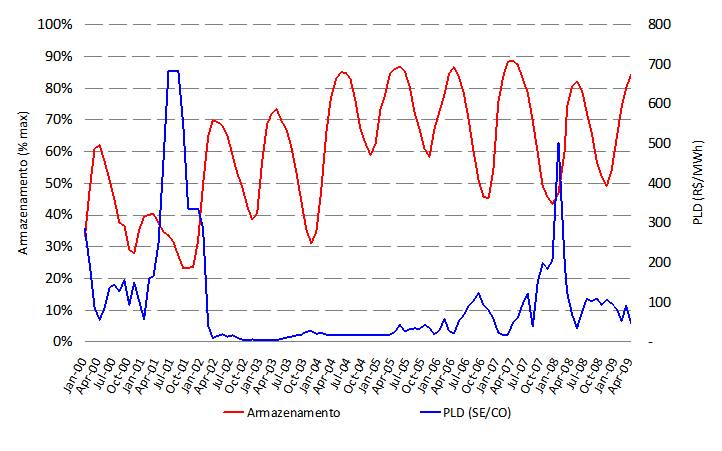
\includegraphics[scale=0.5]{aula9_16}\protect\caption{\label{fig:aula9-16} Curva spot hidrotérmico e armazenamento} 

\end{centering}
\end{figure}
 Para mostrar a receita no spot do gerador hidrelétrico suponha o seguinte perfil de preço spot e geração hídrica apresentados na figura \ref{fig:aula9-17}. 
 \begin{figure}[H]
\begin{centering}
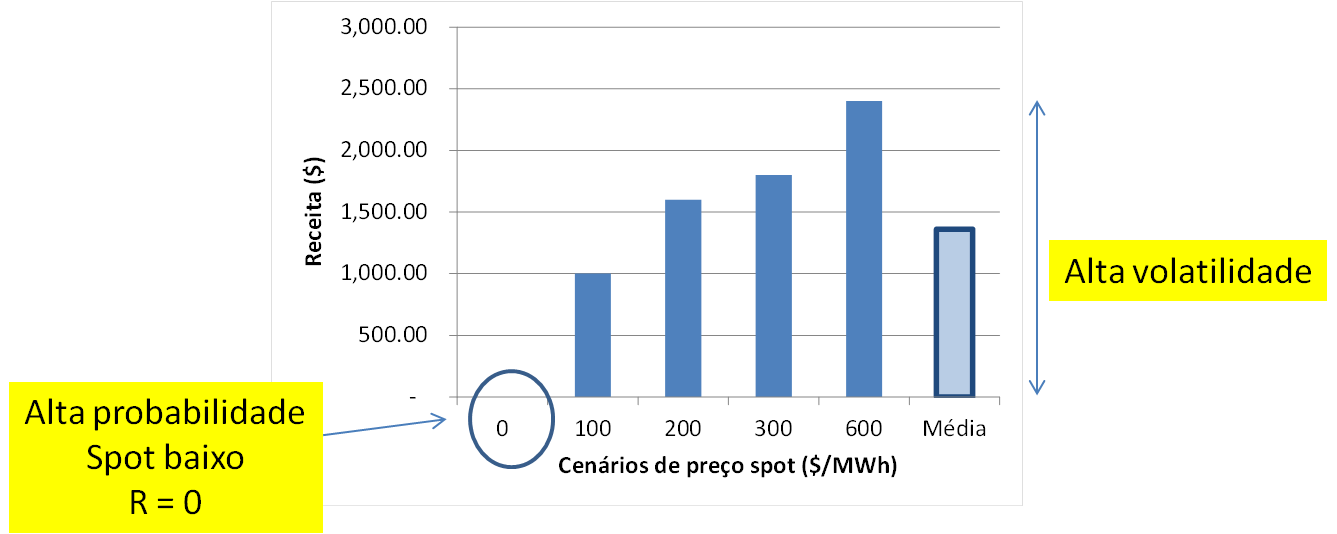
\includegraphics[scale=0.6]{aula9_17}\protect\caption{\label{fig:aula9-17} Curva spot hidrotérmico e armazenamento} 
\end{centering}
\end{figure}

A tabela abaixo apresenta a correlação negativa no sistema elétrico entre preço spot e geração hidrica.
\begin{tabular}{|c|c|c|c|c|c|}
\hline 
cenário & 1 & 2 & 3 & 4 & 5\tabularnewline
\hline 
\hline 
$\pi\$/MWh$ & 0 & 100 & 200 & 300 & 600\tabularnewline
\hline 
$g$$MWh$ & 12 & 10 & 8 & 6 & 4\tabularnewline
\hline 
$R\$$ & - & 1,000.00 & 1,600.00 & 1,800.00 & 2,400.00\tabularnewline
\hline 
\end{tabular}

 Contrato é um acordo bilateral visando garantir receita fixa ou mais instável pra gerador e para o consumidor, ambos tem incentivos.São divididos em financeiros ou físicos, neste curso abordaremos o contrato financeiro. Os contratos financeiros possuem,$Q$: Quantidade em $MWh(MWm\acute{e}dio)$ e $P$: Preço em $\$/MWh$. O vendedor se responsabiliza pela compra de $Q$ em $t$ para o consumidor ao preço $\pi$ er passa a ter um dever no mercado atacadista e o comprador paga ao vendedor $PQ$ e passa a ter o direito a $Q$ no mercado atacadista.  Assim, a receita do gerador passa a ter 3 componentes, a receita fixa do contrato,o dever de compra no mercado da quantidade vendida  e a rceita no mercado da quantidade produzida. Dada por,
 $$R=P\cdot Q-Q\cdot\pi+g\cdot\pi$$.

A receita pode ser vista de duas maneiras,por contratos por diferenças mais clearing da geração($R=(P-\pi)\cdot Q+g\cdot\pi$) e por receita do contrato mais clearing das diferenças($R=PQ+(g-Q)\cdot\pi$),os contratos podem ser firmados com entrega em subsistemas diferentes da geração e será dada por:
$$R=P\cdot Q-Q\cdot\pi_{A}+g\cdot\pi_{B}.$$
 Para verificar a receita no spot do gerador hidrelétrico damos o seguinte exemplo onde o preço de contrato é igual a  média do spot = $240\$/MWh$ e a quantidade de conrato $Q=4MWh$.

 \begin{figure}[H]
\begin{centering}
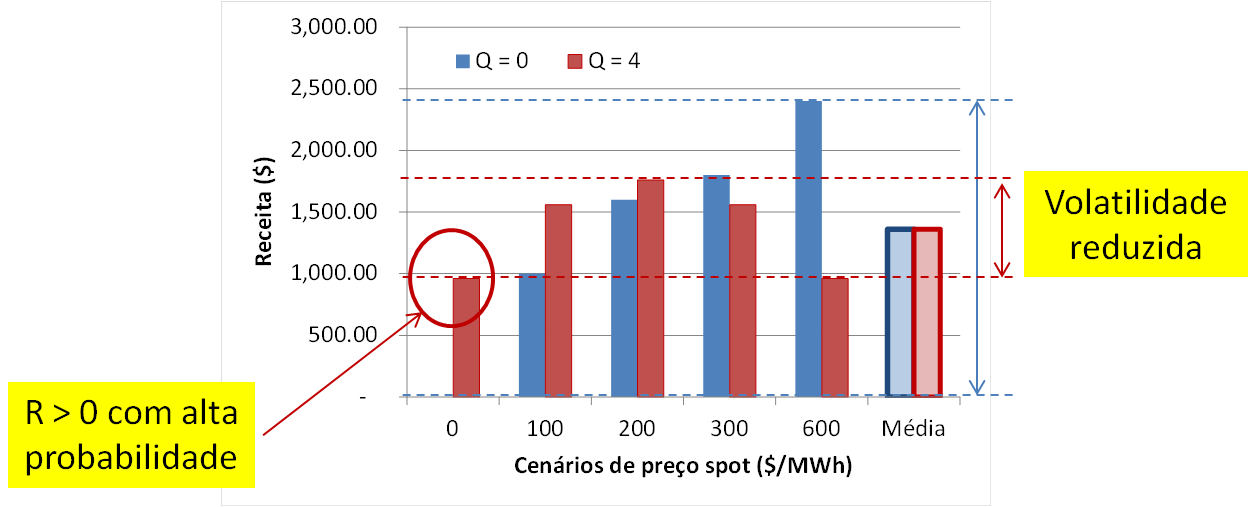
\includegraphics[scale=0.6]{aula9_20}\protect\caption{\label{fig:aula9-20} Exemplo gerador hidrelétrico} 
\end{centering}
\end{figure}

Na figura \ref{fig:aula9-20} é possível verificar a redução da volatilidade ao adicionarmos 4 contratos.

\begin{tabular}{|c|c|c|c|c|c|}
\hline 
cenário & 1 & 2 & 3 & 4 & 5\tabularnewline
\hline 
\hline 
$\pi\$/MWh$ & 0 & 100 & 200 & 300 & 600\tabularnewline
\hline 
$g$$MWh$ & 12 & 10 & 8 & 6 & 4\tabularnewline
\hline 
$R\$$ & 960.00 & 1,560.00 & 1,760.00 & 1,560.00 & 960.00\tabularnewline
\hline 

\end{tabular}

No gráfico \ref{fig:aula9-21} apresenta-se a receita do gerador contratado, considerando a receita média =$1360\$$ e variando a quantidade de contrato em que $Q=1,...,10MWh$. Assim, temos que a quantidade ótima de contratos é de 4.
 \begin{figure}[H]
\begin{centering}
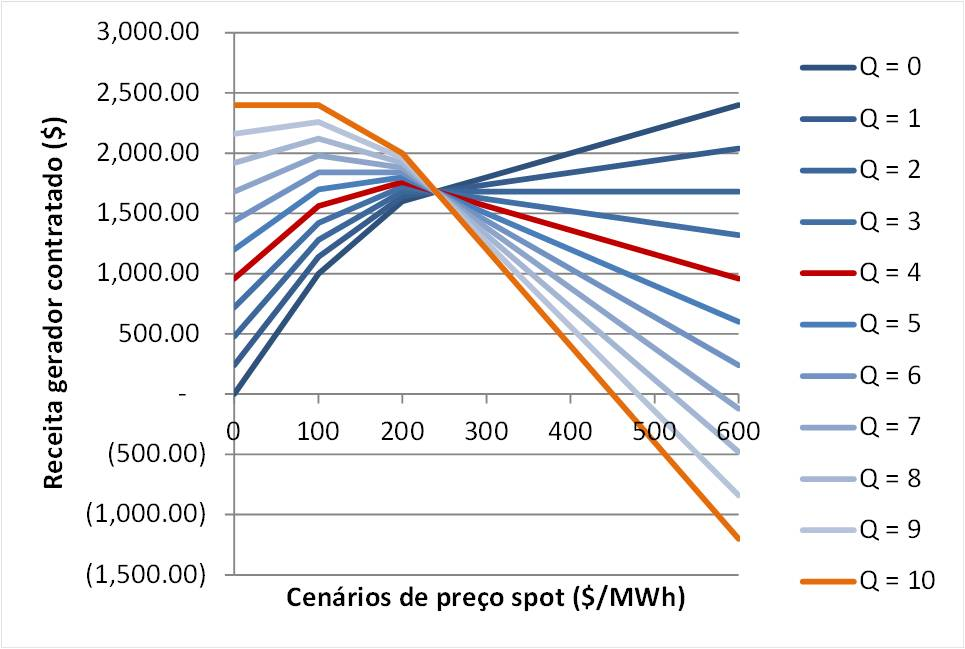
\includegraphics[scale=0.6]{aula9_21}\protect\caption{\label{fig:aula9-21} contratos X receita do gerador contratado} 
\end{centering}
\end{figure}

O gráfico \ref{fig:aula9-22} mostra o menor desvio e o ponto ótimo de contratação, conforme verificado $Q=4$.

 \begin{figure}[H]
\begin{centering}
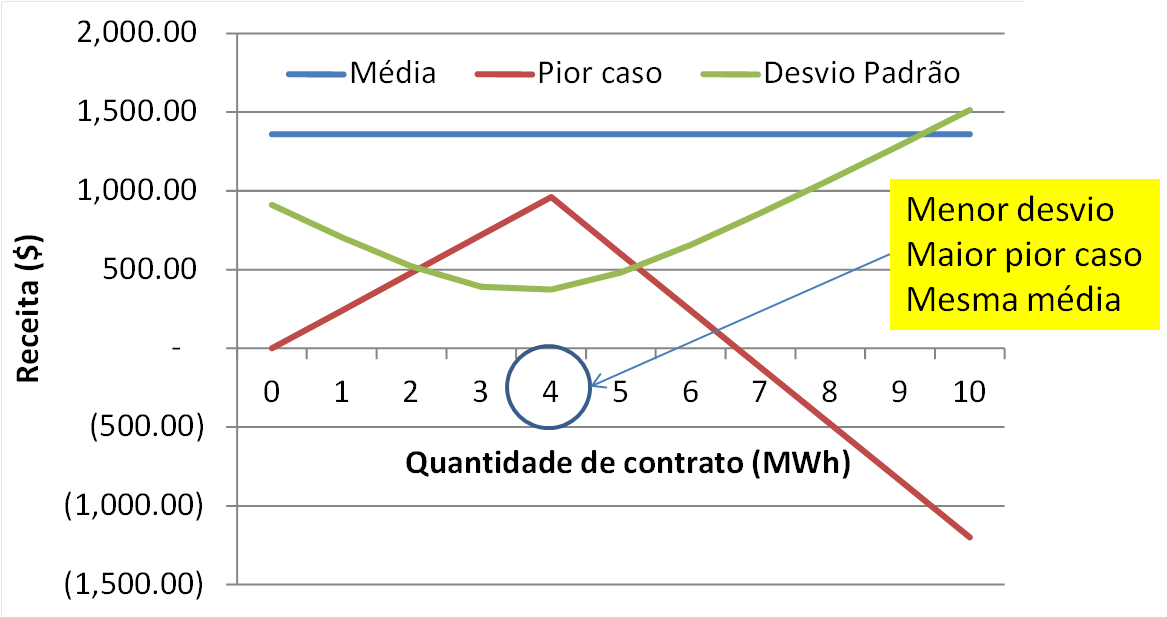
\includegraphics[scale=0.6]{aula9_22}\protect\caption{\label{fig:aula9-22} Contratos ótimos } 
\end{centering}
\end{figure}


Suponha um gerador termelétrico com custo variável igual a $100\$/MWh$
e $G^{max}=10MWh$,vendendo uma quantidade $Q$ $MWh$ à um preço $P=240\$/MWh$.
Temos que,

\begin{tabular}{|c|c|c|c|c|c|}
\hline 
cenário & 1 & 2 & 3 & 4 & 5\tabularnewline
\hline 
\hline 
$\pi\$/MWh$ & 0 & 100 & 200 & 300 & 600\tabularnewline
\hline 
$g$$MWh$ & 0 & 10 & 10 & 10 & 10\tabularnewline
\hline 
R (Q=0) & - & - & 1,000.00 & 2,000.00 & 5,000.00\tabularnewline
\hline 
R (Q=10) & 2,400.00 & 1,400.00 & 1,400.00 & 1,400.00 & 1,400.00\tabularnewline
\hline 
\end{tabular}


 \begin{figure}[H]
\begin{centering}
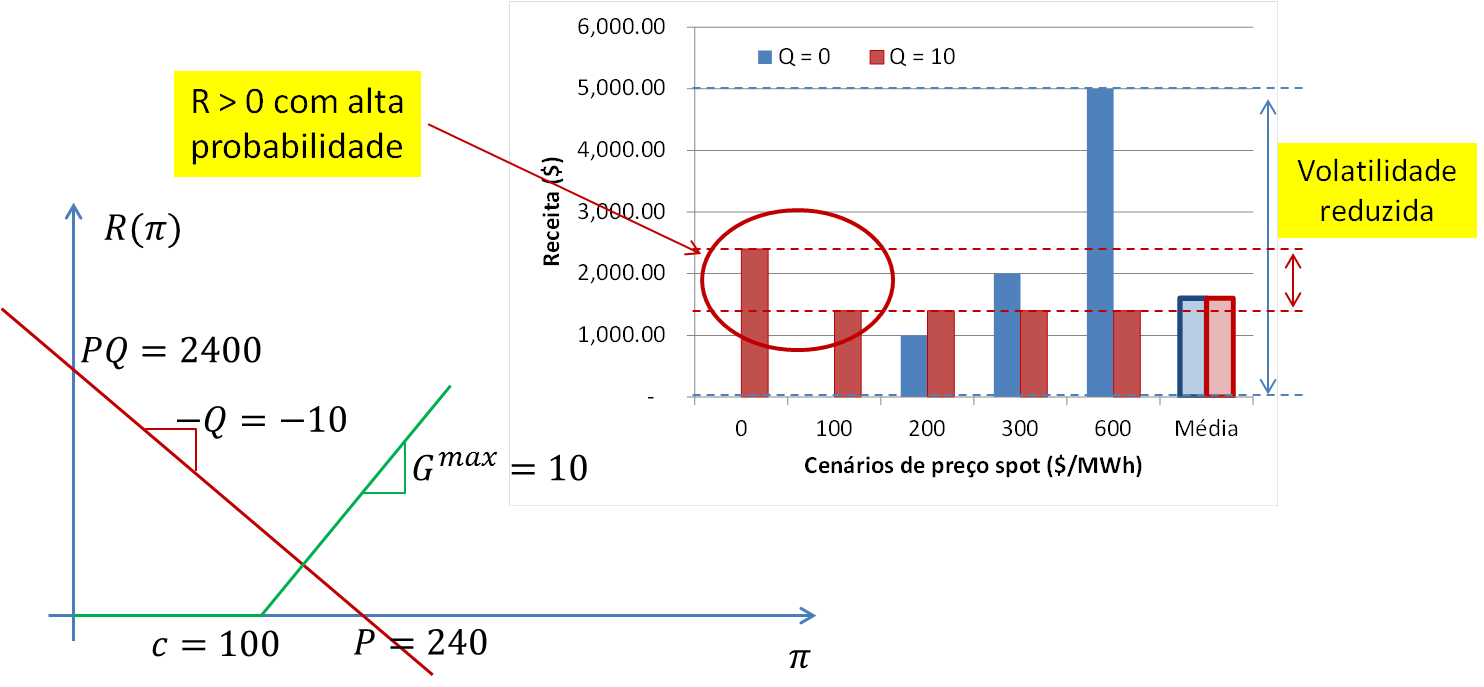
\includegraphics[scale=0.6]{aula9_24}\protect\caption{\label{fig:aula9-24} Gerador térmico } 
\end{centering}
\end{figure}

O contrato reduz a variabilidade da receita

\begin{figure}[H]
\begin{centering}
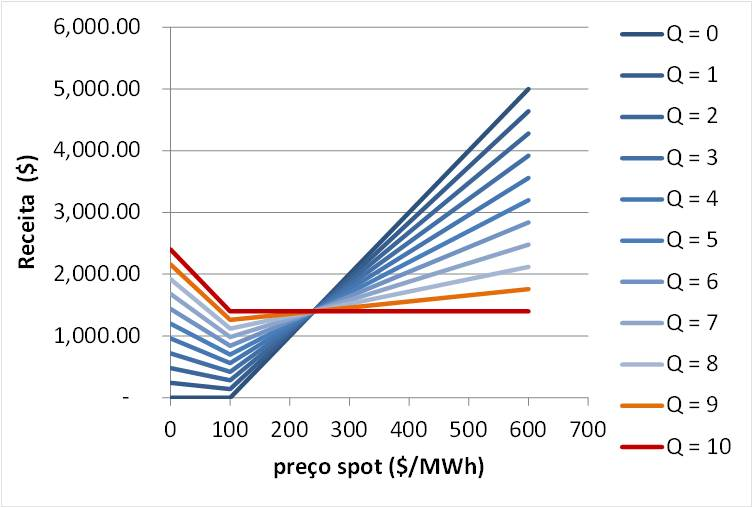
\includegraphics[scale=0.6]{aula9_25}\protect\caption{\label{fig:aula9-25} Contratos ótimio gerador térmico} 
\end{centering}
\end{figure}


Contabilização no mercado atacadista com contratos
\begin{figure}[H]
\begin{centering}
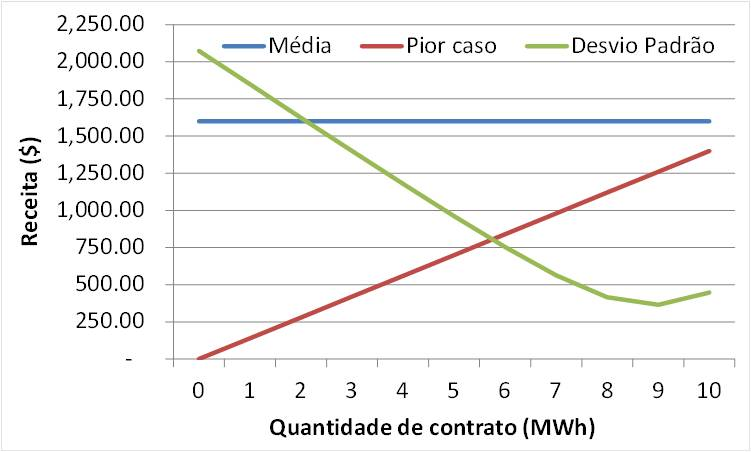
\includegraphics[scale=0.6]{aula9_26}\protect\caption{\label{fig:aula9-26} Curva de observação da quantidade ótima de contratação } 
\end{centering}
\end{figure}

Suponha que agora que naquele exemplo da linha de transmissão G1 vende para $D2:9MWh$ a $10R\$/MWh$ e G3 vende para $D1:5MWh$ a $20R\$/MWh$. Assim, a operação não é alterada pelos contratos figura \ref{fig:aula9-27}.

\begin{figure}[H]
\begin{centering}
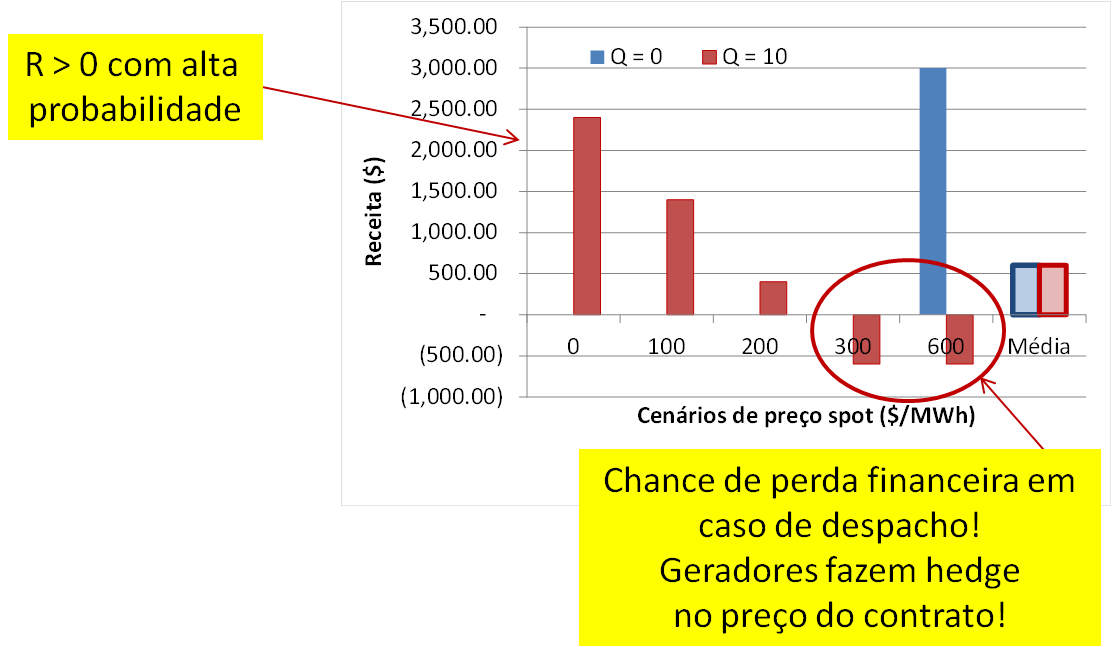
\includegraphics[scale=0.6]{aula9_27}\protect\caption{\label{fig:aula9-27} Gerador térmico} 
\end{centering}
\end{figure}
 
\begin{tabular}{|c|c|c|c|c|c|c|c|}
\hline 
Gerador: Consumidor: & Quantidade contratada Q MWh & Geração ou consumo $g-D$ MWh & Spot $\pi$$\$/MWh$ & Receita no spot $g\pi-D\pi$ $\$$ & Receita Liquidação $(g-Q)\times\pi(Q-D)\times\pi$$\$$ & Receita com contrato $QP$$\$$ & Receita Total $PQ+(g-Q)\pi-PQ+(Q-D)\pi$ $\$$\tabularnewline
\hline 
\hline 
$G_{1}$ & -9 & 10 & 12 & 120 & $1\times12=12$ & $9\times10=90$ & 102\tabularnewline
\hline 
$G_{2}$ &  & 4 & 12 & 48 & $4\times12=48$ &  & 48\tabularnewline
\hline 
$G_{3}$ & -5 & 0 & 12 & 0 & $-5\times12=-60$ & $5\times20=100$ & 40\tabularnewline
\hline 
$D_{1}$ & 5 & -3 & 12 & -36 & $2\times12=24$ & $-5\times20=-100$ & -76\tabularnewline
\hline 
$D_{2}$ & 9 & -11 & 12 & -132 & $-2\times12=-24$ & $-9\times10=-90$ & -114\tabularnewline
\hline 
Fechamento & 0 & 0 & 12 & 0 & 0 & 0 & 0\tabularnewline
\hline 

\end{tabular}

Mecanismos de mercado e expansão

Contratos mitigam o risco de receita baixa,proporcionam garantias para obter taxas mais atrativas de financiamento. Diversos mecanismos são utilizados para se estabelecer contratos dependendo das características do sistema, o day ahead market (pool) que são contratos de 1 hora para cada hora do dia seguinte  e estabelecidos através de modelos complexos como o unit commitment, restrições de rede e segurança. Ouro mecanismo é o ambiente de contratação regulado onde os  contratos de 1, 15, 20 e 30 anos com contabilização semanal e  estabelecidos através de leilões iterativos híbridos entre
preço uniforme decrescente, seguido de rodada final pay as bid.
